\documentclass{article}

\usepackage{amsmath,amssymb,amsthm}

\usepackage{graphicx}
\graphicspath{ {./img/} }

\usepackage{biblatex}
\addbibresource[
    style=authoryear
]{resources.bib}

\newtheorem{thm}{Theorem}
\newtheorem{def}{Definition}
\newtheorem{rk}{Remark}
\newtheorem*{variants}{}
\newtheorem*{var}{}

\renewcommand{\Rn}[1][n]{\mathbb{R}^{#1}}
\newcommand{\Absbars}[1]{\left\lVert#1\right\rVert}
\newcommand{\rmfd}[1]{Riemannian manifold}

\title{Ch. 12: The Energy of a Path}
\author{Nicolas Trutmann}
\date{}

\begin{document}
\maketitle


We'll prove what would seem intuitive, namely that geodesics are minima of both length and energy of
a path between 2 points. That is the project we're working towards.

that was kind of the point of geodesics in the first place. They were defined with the intent of
making a 'minimal path' between two points; an analogue of the straight line in $\Rn$.

Let's give a definition:

\begin{def}[Energy of a Path]
Let $\omega : \Rn[] \rightarrow M $ be a path on a \rmfd, with $\omega(a) = p$ and $\omega(b) = q$.
I.e. $\omega \in \Omega_{p,q}(M)$
\[ E_a^b(\omega) = \int_a^b \Absbars{\frac{d\omega}{dt}}^2 dt \]

We leave off the indices for curves parametrized on $[0,1]$, so $E = E_0^1$.
\end{def}


\begin{def}
\label{def:vel_of_var}
    The velocity of a variation $\alpha: (-\epsilon, \epsilon) \rightarrow \Omega(M;p,q)$ with
    $\alpha(0) = \omega$ is defined as

    \[ W_t = \frac{d\alpha}{du}(0)_t = \]

    It is the vector field along $\omega$ with $W \in T\Omega_{\omega}$.
\end{def}


\subsection{the proportional to arclength argument}

a problem with curves is that we could parametrize them arbitrarily badly.

\begin{def}
    \label{def:reparametrization}
    We say a curve $\gamma$ is
\end{def}


\subsection{sleight of hand: calculus of variations}

\newcommand{\OM}{\Omega(M)}
The big cheat of these chapters is that we're able to do calculus on $\OM$.
This is a priori not a manifold, topological space, vector field or group.
It becomes, however, after doing some math to it.

In Milnor's book \cite{milnor}, this problem is explicitly brushed under the table.
Books that treat the matter more thoroughly brush it under the table with a few more words
\cite{salamon}.
Here is a reference that is explicit and thorough: \cite{lee}

Since Milnor hand-waves the problem, so will we. Since we still need intuition for what we're
skipping I provide here two pictures, which we will pretend is how all the curves under scrutiny
look like.

\begin{figure}
    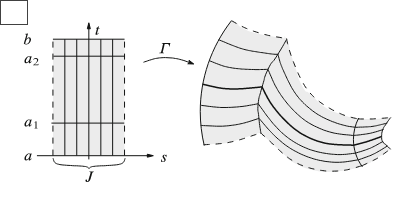
\includegraphics{img/grid.png}
    \caption{grid shape}
    \label{fig:boat1}
\end{figure}
\begin{figure}
    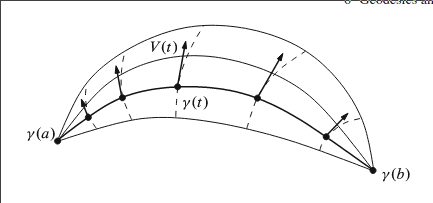
\includegraphics{img/sail.png}
    \caption{variation}
    \label{fig:boat1}
\end{figure}


\subsection{The Characterization Theorem}

\begin{thm}[Characterization of Geodesics]

    Let $I = [a, b] \subset \Rn[]$ be a compact interval and let $\gamma : I \rightarrow M$ be a
    smooth curve. Then the following are equivalent.

    \begin{enumerate}
    \item γ is an extremal of the energy functional, i.e. every variation {γs}s∈R
        of γ with fixed endpoints satisfies
        d
        ds
        ∣
        ∣s=0 E(γs) = 0.
    \item γ is parametrized proportional to the arclength, i.e. the veloc-
        ity |  ̇γ(t)| ≡ c ≥ 0 is constant, and either γ is constant, i.e. γ(t) = p = q for
        all t ∈ I, or c > 0 and γ is an extremal of the length functional, i.e.
        every variation {γs}s∈R of γ with fixed endpoints satisfies
        d
        ds
        ∣
        ∣s=0 L(γs) = 0.
    \item The velocity vector of γ is parallel, i.e. ∇  ̇γ(t) = 0 for all t ∈ I.
    \item The acceleration of γ is normal to M , i.e.  ̈γ(t) ⊥ Tγ(t)M for all t ∈ I.
    \end{enumerate}


\end{thm}



\subsection{Examples and edgecases}


Hyperbolic space

Projective space


\printbibliography

\end{document}
